\section{Day 3: Logical Devices (Sep 16, 2025)}

To avoid having to deal with gates, we gain another level of abstraction through circuits, which are more complex structures. These include multiplexers (aka mux), decoders, adders (half and full), subtractors, and comparators.

\begin{definition}[Combinational Circuit]
A circuit where the output strictly relies on the inputs.
\end{definition}

Another category is \textit{sequential circuits} which we will learn about later, which rely on memory. De-multiplexers may be testable, implement one in your own time.

Decoders are translators, which translates the output of one circuit to the input of another. A 7 segment decoder, aka a 7 segment is active-high, meaning that a segment is on when its input is high, and off when its input is low. Active-low also exists, mainly used for safety purposes.

In a Karnaugh map, undefined inputs are represented by an \texttt{x}. We do not care about this value, we can make it 0 or 1, whichever to achieve a simpler expression (bigger rectangles = simpler expressions). Karnaugh maps are not a proof technique, they are a somewhat quick and dirty way to get a simple looking expression. 

\begin{remark}
If you are so \textit{talented} that you can immediately identify the simplified expression, the steps are NOT for you. You wouldn't need them anyway. - Prof
\end{remark}

\subsection{Adder Circuits}

Aka binary adders, they are circuit devices that add two digits together. There exist half and full adders. Single digit unsigned binary addition is straightforward, which we capture using a half adder:

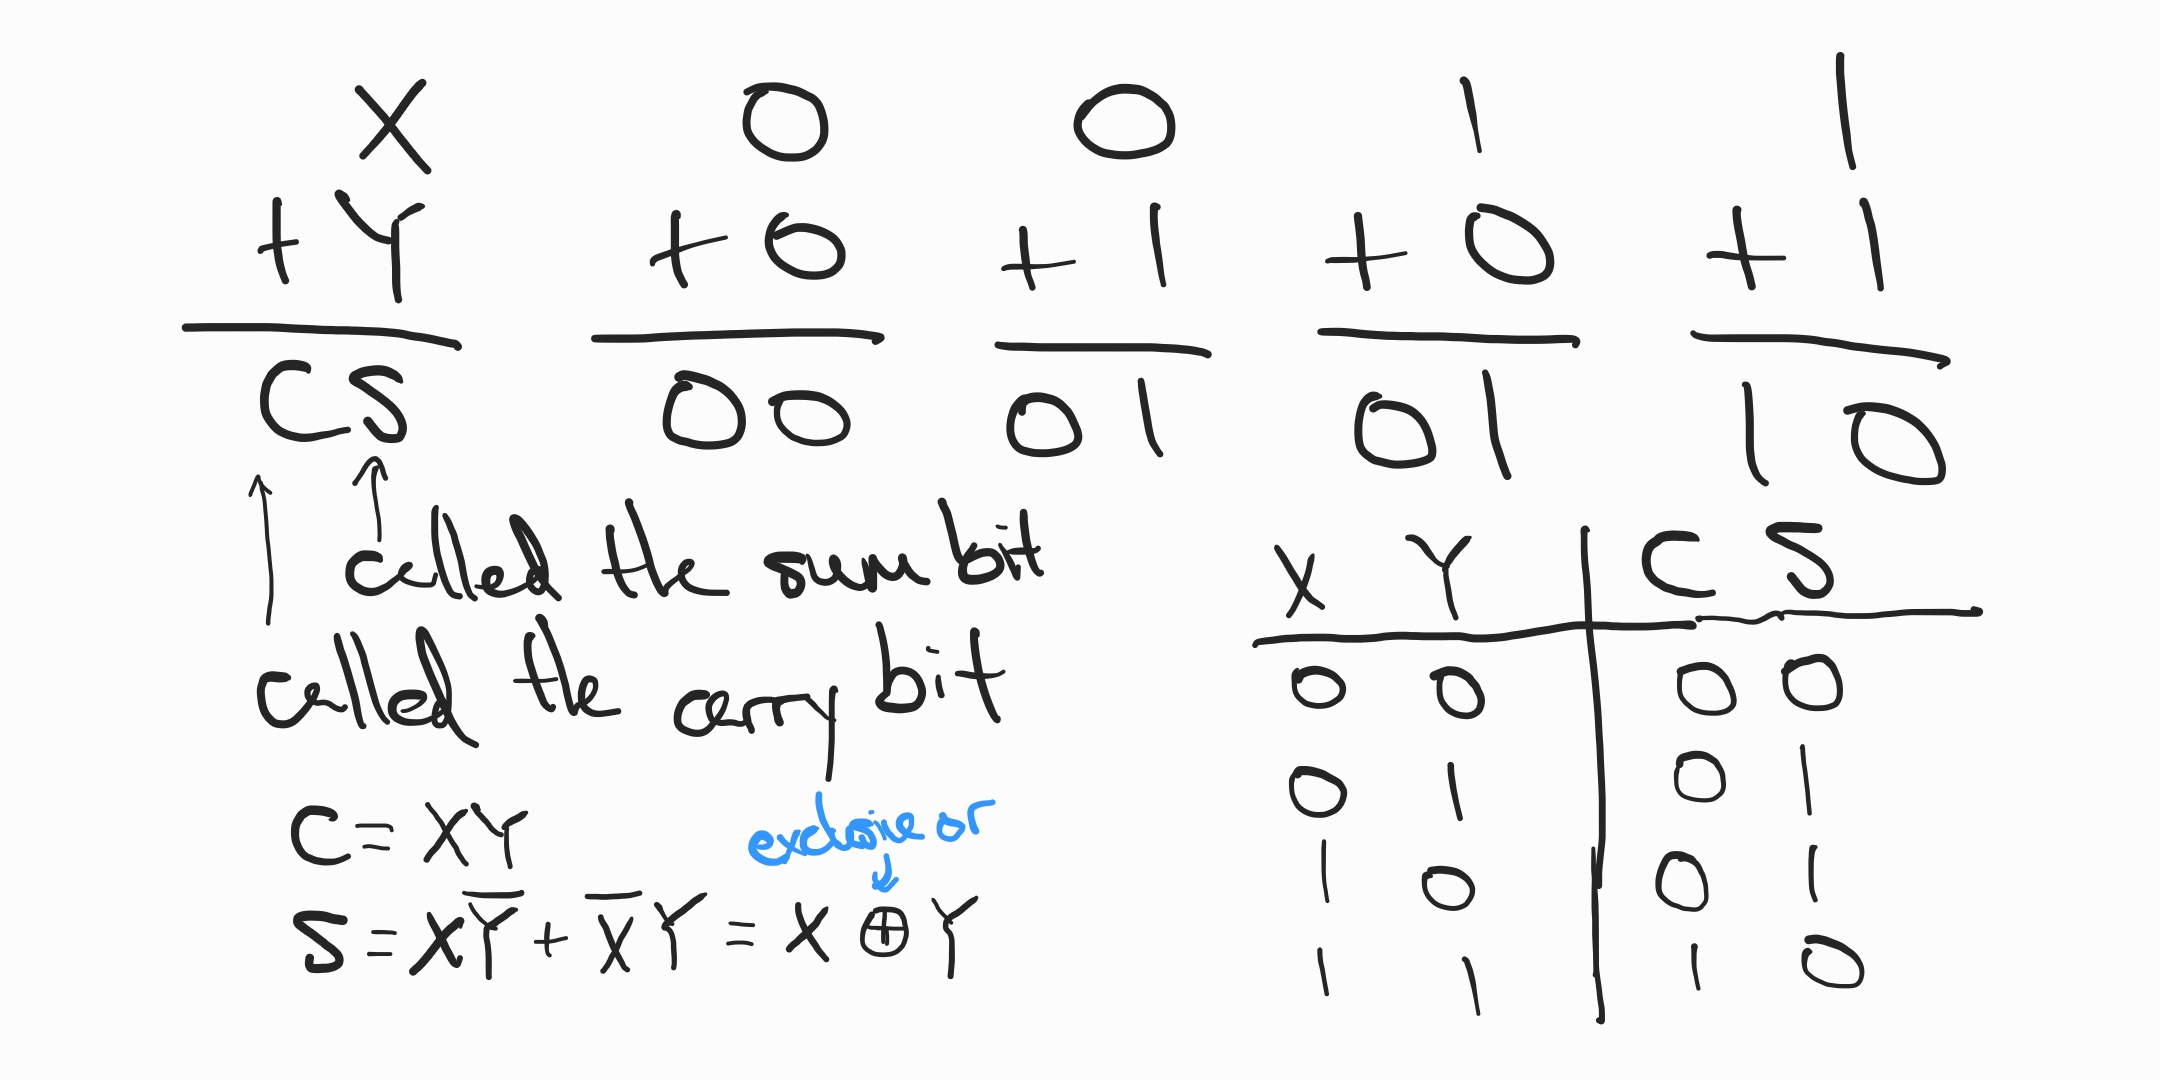
\includegraphics{csc258/figures/halfadderttb.jpg}

To account for the carry, we need potentially sum up 3 numbers! A full adder has inputs $X, Y, Z$ and outputs $C, S$. When $Z$ is 0, it behaves identically to a full adder. A full adder takes into consideration the carry of the sum of the previous two digits.

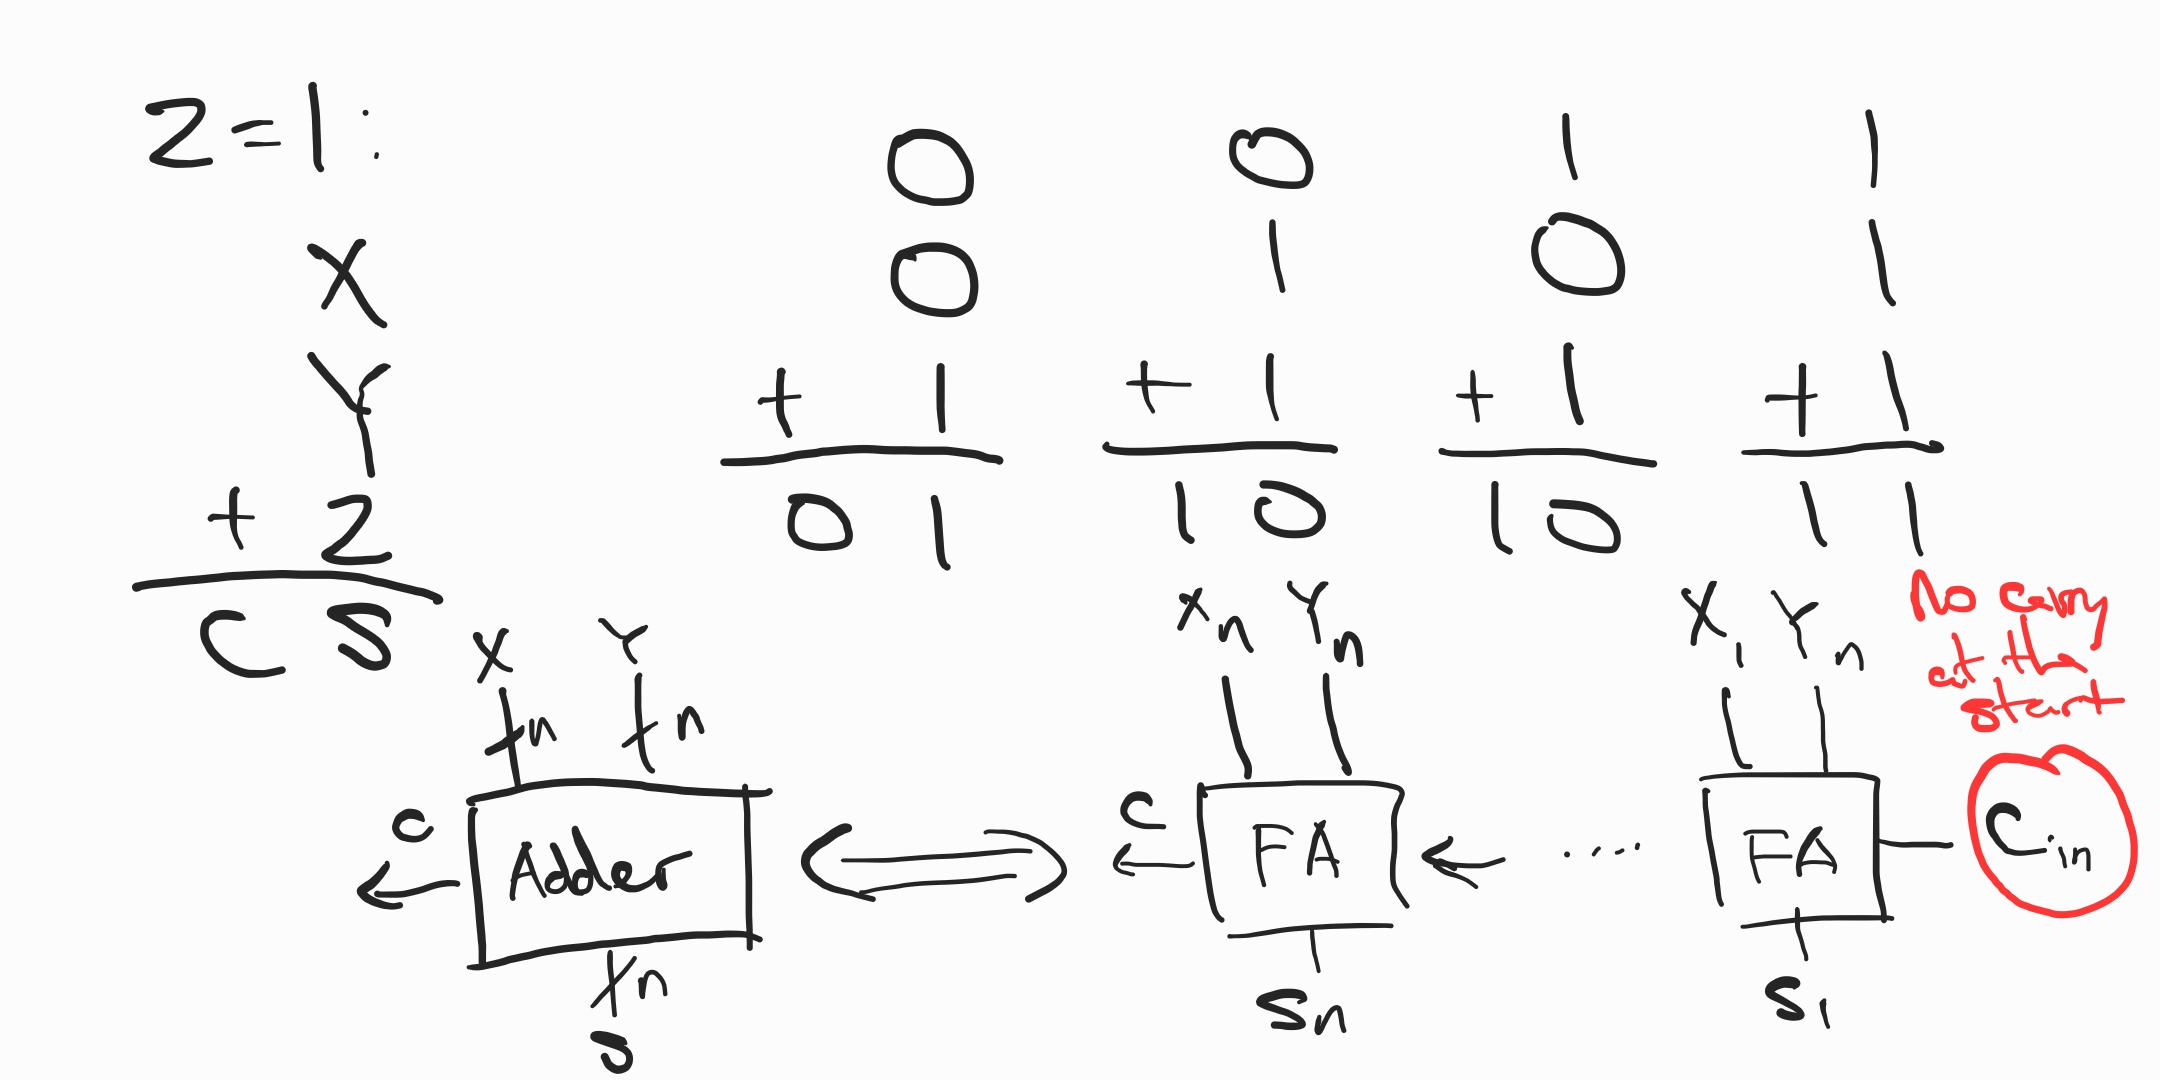
\includegraphics{csc258/figures/fulladder.jpg}

As shown in the diagram, to make use of the carry functionality provided by the full adder, we join them together to compute the sum of two $n$ digit numbers, though you do also need to consider the carry.

Now that we have an adder, we should look into subtraction. Recall that a negative integer is the additive inverse for a positive integer, meaning $(-a) + a = 0$.

When you flip all of the bits of a int, the number you obtain is called one's complement. When you add one to one's complement, you get \textit{two's complement}. While using two's complement, to distinguish negative numbers from positive numbers we need to keep track of a sign-bit, typically the most significant bit. With a $n$-bit computer, you can only keep track of as big of a positive integer as a $(n-1)$-bit computer can.

Remember that in an adder circuit, $c_{in}$ is unused, but we can reuse this feature in our subtractor circuit, where for two's complement need to flip all the bits for a number and add one, which $c_{in}$ can do.

\subsection{Comparator}

Comparators are crucial, they are used extremely often and are used to inform decisions. Comparators take two input vectors, and determines which one is bigger than or equal to the other. Recall that for any 2 integers $A, B$, exactly one of $A = B$, $A > B$, $A < B$ is true. We can implement a one bit comparator as follows:

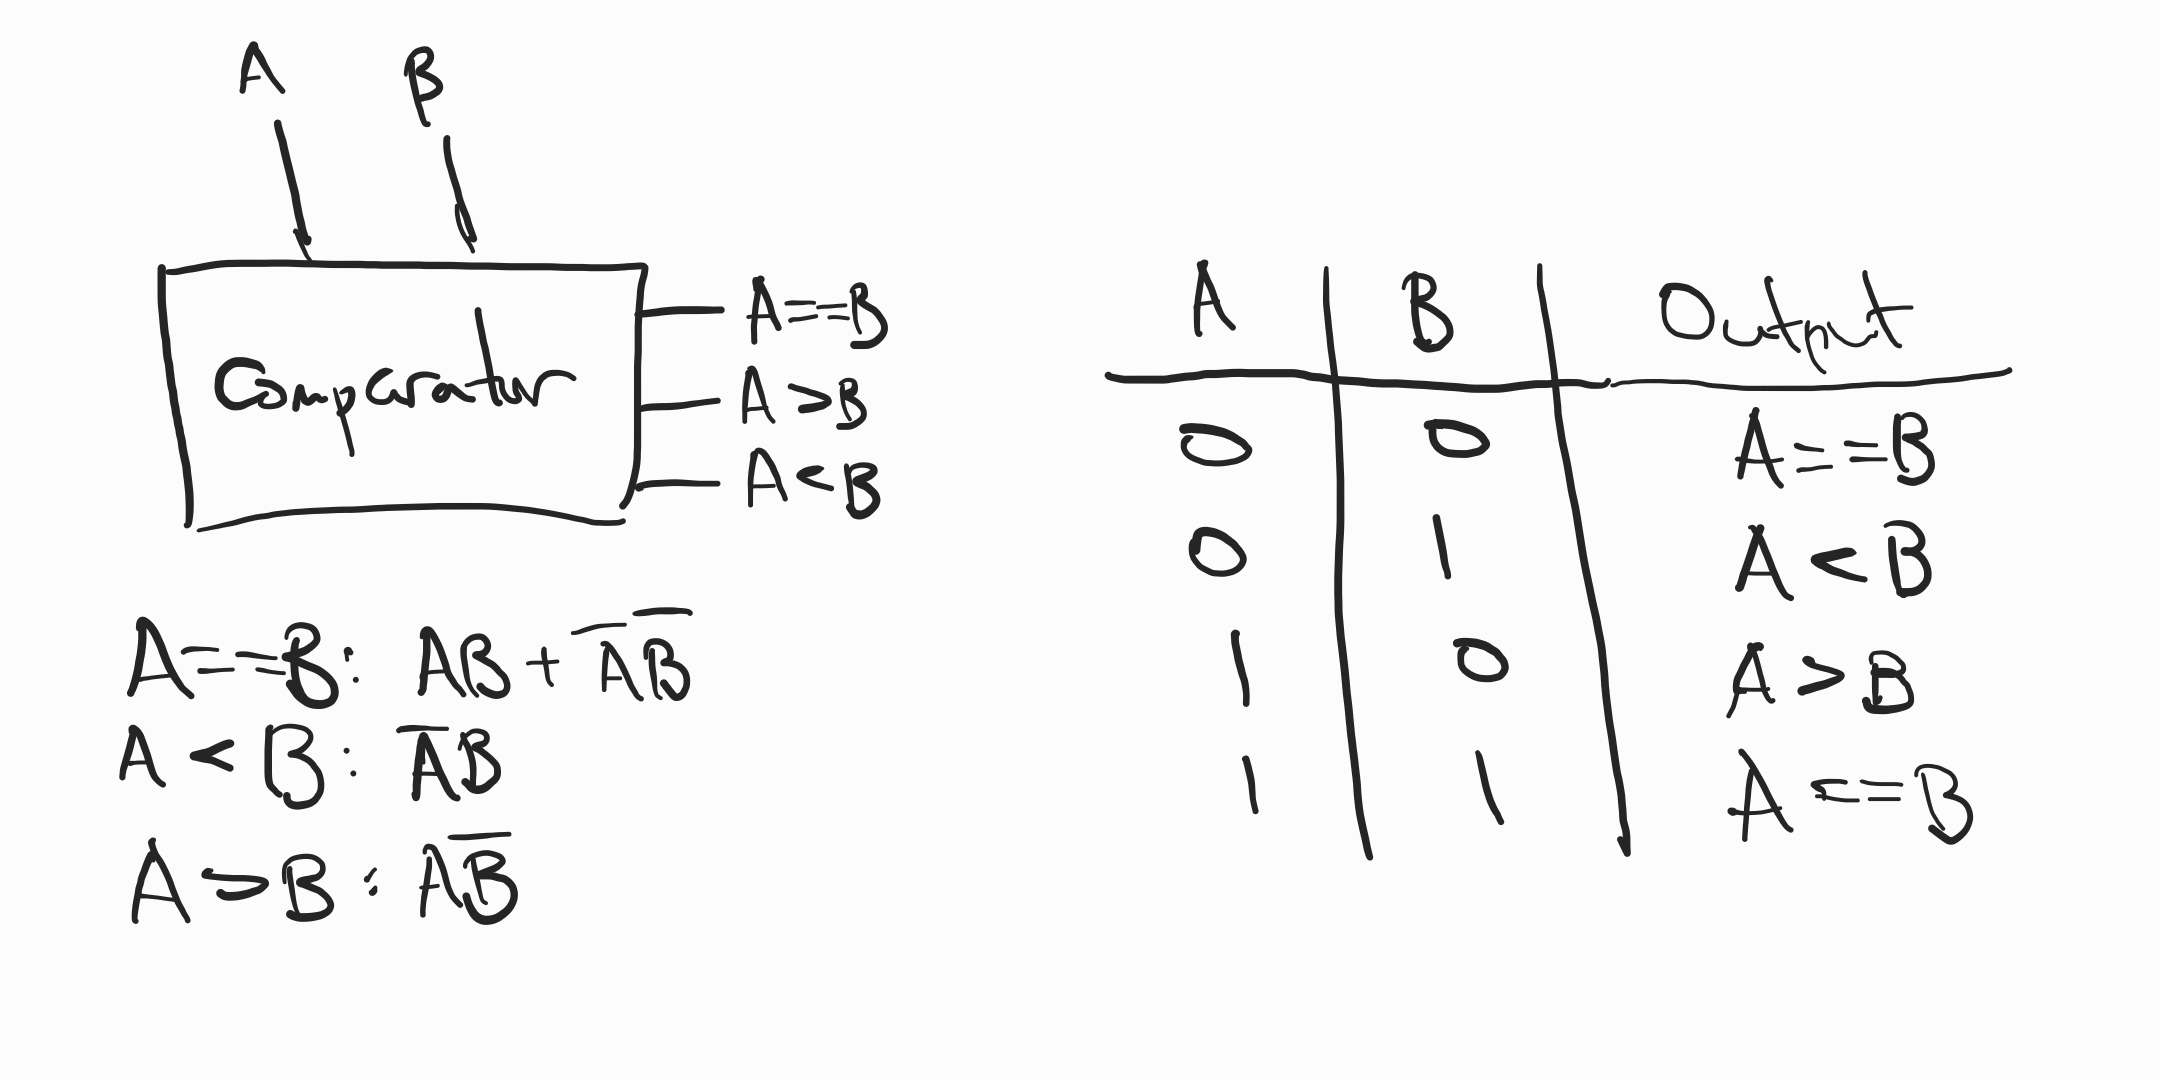
\includegraphics{csc258/figures/1bitcomparator.jpg}

\begin{exercise}
Generalize to a $n$-bit comparator. 
\end{exercise}

\begin{exercise}
Create a circuit that supports both addition and subtraction of $n$-digit binary numbers.
\end{exercise}

\subsection*{Lab Info}

In the first part of the lab you will learn to make your designs modular, and create a 4-to-1 mux using 2-to-1 muxes.

In the second part of the lab you will be dealing with a field programmable gate array (FPGA), which is like a CPU, but you can re-wire it in the field. It gives you control over some gates. For our lab, the 7 segment display that we'll be working with is \texttt{HEX0}, which is the rightmost one. We're also concerned with the switches and LEDs, through which we handle input. \textbf{The DE1-SOC board is active-low}.

